%PIP-412035RC020
\documentclass[reprint,amsmath,amssymb,aps,prb,footinbib,floatfix]{revtex4-2}
\bibliographystyle{apsrev4-2}
\usepackage{afterpage}
\usepackage{blindtext}
\usepackage[rgb]{xcolor}
%\usepackage[twocolumn=true,includehead=false,left=.75in,right=.75in,top=.75in,bottom=.75in]{geometry}
%\usepackage[letterpaper, portrait, twocolumn, twoside, left=2cm, hmarginratio=2:1, includemp, marginparwidth=43pt, bottom=1cm, foot=.7cm, includefoot, textheight=11cm, heightrounded, columnsep=1cm, dvips, verbose]{geometry}
\definecolor{Cred}{RGB}{208, 32, 46}
\usepackage[firstpage=true]{background}
\usetikzlibrary{calc}
%\usepackage{tikz}
\backgroundsetup{angle = 0, scale = 1, vshift = 0pt, opacity=1,
  contents = {\begin{tikzpicture}[overlay,remember picture]
    \node at (0,0) {\includegraphics[scale=1]{RC_def.pdf}};
\end{tikzpicture}
}
}
%    \draw (3.4in,3.75in) node[inner sep=0] {\includegraphics[width=1in]{arrow.pdf}};
%    \draw (3.5in,3.85in) node[rotate=-90] {\scshape{Editor's}};
%    \draw (3.5in-\baselineskip,3.85in) node[rotate=-90] {\scshape{Suggestion}};
%\end{tikzpicture}

\usepackage{graphicx} % Required for inserting images
\usepackage{mathtools} % Useful for a bunch of math stuff
\usepackage{cleveref} % Use for better cross-references
\usepackage[caption=false]{subfig} % For sub-figures
\usepackage{booktabs} % For nicer looking tables
\usepackage[twoside]{fancyhdr}
\usepackage{appendix}

\usepackage{placeins}




\fancypagestyle{plain}{%
%\setlength{\headheight}{60pt}
\fancyhead[L,C]{}
\fancyhf{}
\fancyhead[R]{\raisebox{.6cm+1pt}{\textbf{Rapid Communication}}}
\fancyhead[L]{ \raisebox{.6cm+1pt}{\scshape{Editor's Suggestion}\vspace{12pt}}}
\fancyhead[C]{\raisebox{.6cm}{\large\scshape{CARTHAGE}}\hspace{0.2cm}\includegraphics[height=1.5cm]{Logo.pdf}\hspace{0.1cm}\raisebox{.6cm}{\large\scshape{COLLEGE 
 }}}
\fancyfoot[C]{\thepage}
\renewcommand{\headrulewidth}{0pt}
\renewcommand{\footrulewidth}{0pt}
}
\usepackage{printlen}


\pagestyle{fancy}
\fancyhf{}
\fancyheadinit{\setlength{\headheight}{20pt}}
\fancyhead[RO,LE]{\textbf{Rapid Communication}}
\fancyhead[LO,RE]{\textit{Phys. in Prog.} \textbf{2} (Feb. 2026)}
\fancyhead[C]{ \large \scshape{PHYSICS IN PROGRESS}}
\fancyfoot[C]{\thepage}
\renewcommand{\headrulewidth}{0.4pt}
\renewcommand{\footrulewidth}{0pt}

% These are packages I am using in this document
\usepackage{siunitx}

% Everything up to here is the 'document preamble'

\begin{document} 

\vspace*{25pt}




\title{Getting swingy with it: 
determining gravity using a simple pendulum}
\author{Brookelyn H. Velmont}
\affiliation{%
Department of Physics and Astronomy,  Carthage College, 2001 Alford Park Drive, Kenosha, WI 53140, USA
}%
\collaboration{Received January 29, 2026, Published online February 5, 2026}
\affiliation{Department of Physics and Astronomy, Carthage College, 2001 Alford Park Drive, Kenosha, WI 53140, USA}
\begin{abstract}
This experiment uses a simple pendulum to measure the acceleration due to gravity. This is done by timing the pendulum's oscillations for several different string lengths. For small release angles, the motion of the pendulum can be approximated as simple harmonic motion, leading to the linear relationship between the period of oscillation and the square root of the length of the pendulum. The time for ten oscillations was measured for multiple trials for ten different lengths. A weighted linear fit of period versus the square root of length was used, whose slope was proportional to g. This gave $g=10.01\pm0.04m/s^2$. This value is slightly larger than the accepted value, likely due to systematic timing uncertainties. The results clearly follow the expected linear relationship.
\end{abstract}
\maketitle
\section{Introduction}

Despite their apparent simplicity, pendulums have been important tools in physics for centuries, from Galileo’s early observations of regular motion in swinging chandeliers to Foucault’s use of a large pendulum to demonstrate Earth’s rotation. Galileo’s work on isochronism laid the foundation for the development of accurate timekeeping, and Christiaan Huygens later developed pendulum clocks, which greatly improved navigation and measurement.

A simple pendulum consists of a mass suspended from a fixed point by a light string. When displaced from equilibrium and released, the pendulum swings back and forth under the influence of gravity, with a restoring force directing it toward equilibrium. For small angular displacements, the motion is approximately periodic, and the period depends primarily on the length of the pendulum and the acceleration due to gravity \cite{belendez2007exact}. Real pendulums deviate from the ideal due to air resistance, friction, and the finite mass of the string, providing an opportunity to explore the limitations of theoretical models and the role of experimental uncertainty.

In this experiment, the period of a simple pendulum was measured for several string lengths to investigate the relationship between oscillation period and pendulum length to determine the acceleration due to gravity. By analyzing how the period changes with length, this study demonstrates the principles of simple harmonic motion while highlighting experimental limitations. Even with simple equipment, the experiment illustrates how classical mechanics can be connected to hands-on observations, making it accessible for both educational and research purposes.

\section{Key Findings}
\begin{figure}
    \centering
    \includegraphics[ width=0.8\linewidth] {drawing.pdf}
    \caption{Diagram of experimental setup, showing simple pendulum with mass $m$, length $L$, and small angle $\theta$. }
    \label{fig:pendulum}
\end{figure}

A simple pendulum is a system consisting of a point mass $m$ suspended from a fixed pivot by a massless, inextensible string of length $L$. When displaced from its equilibrium position and then released, the pendulum swings back and forth due to the force of gravity. The force of gravity acts vertically on the mass, and only the component of this force along the arc of motion contributes to restoring the pendulum toward its equilibrium. This component of the gravitational force creates a restoring torque about the pivot that returns the pendulum to its lowest point.

The restoring torque $\tau$ is related to the angular displacement $\theta$ from equilibrium:
\begin{equation}
\tau=mgL\sin\theta,
\end{equation}
where the negative sign indicates that the torque acts against the displacement. The torque generates angular acceleration $\alpha$ according to Newton’s second law for rotation:
\begin{equation}
\tau=I\alpha,
\end{equation}
where $I=mL^2$ is the moment of intertia of the mass about the pivot, and $\alpha=d^2/\theta dt^2$ is the angular acceleration. Therefore, the angular displacement of the pendulum satisfies the nonlinear equation: 
\begin{equation}
\frac{d^2\theta}{dt^2}+\frac{g}{L}\sin\theta=0.
\end{equation}
For small angular displacements, $(\theta \leq \SI{15}{\degree})$, $\sin\theta=\theta$. This small-angle approximation linearizes the equation, making it mathematically equivalent to a simple harmonic oscillator. Physically, this means the restoring torque is approximately proportional to the displacement, which results in periodic motion with a fixed frequency. The resulting linear differential equation is:
\begin{equation}
\frac{d^2\theta}{dt^2}+\frac{g}{L}\theta=0,
\end{equation}
a second-order ODE whose solution has two constants of integration representing the initial amplitude and phase. The angular frequency is
\begin{equation}
\omega=\sqrt{\frac{g}{L}}.
\end{equation}
The period of oscillation, $T=2\pi/\omega$, is now
\begin{equation}
T=2\pi\sqrt{\frac{L}{g}}.
\end{equation}
This predicts a linear relationship between $T$ and $\sqrt{L}$.



The experimental apparatus shown schematically in Fig. \ref{fig:pendulum} consisted of a simple pendulum formed by a spherical metal mass suspended from a fixed support by an inextensible string of negligible mass. The string was attached to a fixed rod supported by the edge of a rigid horizontal surface, forming a fixed pivot point about which the pendulum oscillated. The pendulum length $L$ was defined as the distance from the pivot point to the center of mass of the metal sphere. 

Oscillations began with a small angular displacement $\theta=\SI{10}{\degree}-\SI{15}{\degree}$ to satisfy the small-angle approximation. Three different string lengths were used while the mass of the pendulum was held constant. For each length, the time for ten complete oscillations was measured using a handheld stopwatch. Each measurement was repeated three times and averaged to reduce random timing uncertainty. 

\begin{figure}
    \centering
    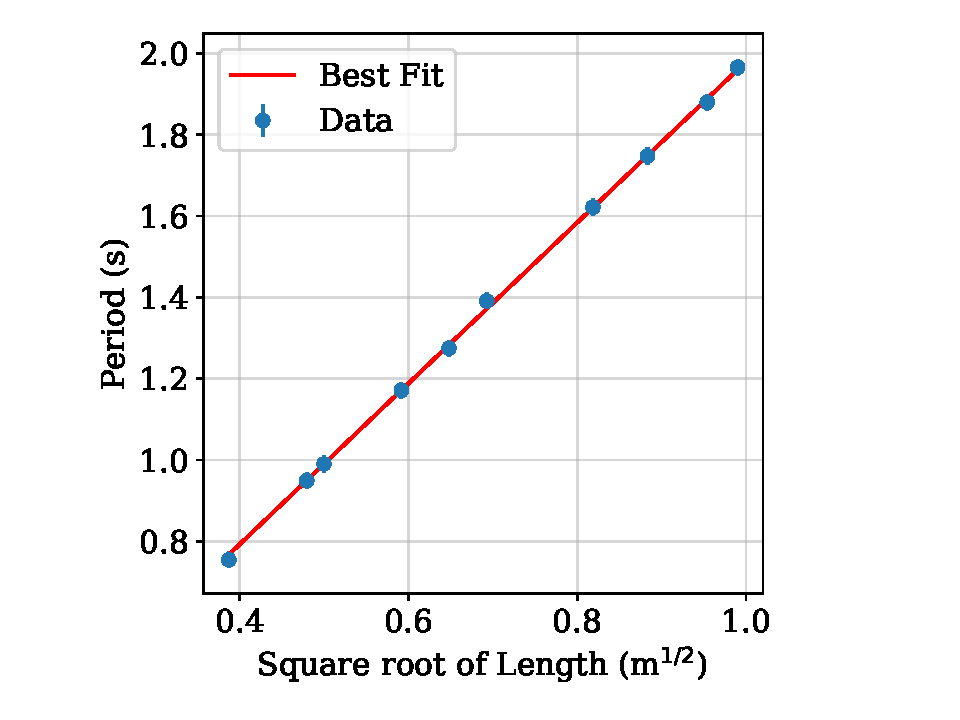
\includegraphics[ width=\linewidth] {gravity.pdf}
    \caption{The average of the measured periods is plotted against the square root of the measured lengths. The solid line is a least squares regression fit. }
    \label{fig:plot}
\end{figure}

The plot of measured values for the period versus the square root of the pendulum length is shown in Fig. \ref{fig:plot}. A weighted linear regression was performed, forcing the fit through the origin, consistent with the theoretical relationship $T \alpha \sqrt{L}$. The slope of this line, $M$, represents a ratio of $2\pi$ to $g$. Rearranging this ratio gives the calculated value of gravitational acceleration:
\begin{equation}
g = 10.07 (2M)^2  \pm 0.04 \ \mathrm{m/s^2}.
\end{equation}
The accepted value of gravitational acceleration is 
\begin{equation}
g_{\mathrm{accepted}} = 9.80665 \ \mathrm{m/s^2},
\end{equation}
as reported in \cite{nist_gn}.
The experimentally determined value differs from the accepted value by $2.6\%$.

Despite this small discrepancy, the data clearly demonstrates the expected linear dependence of period on the square root of length. The slight overestimation of g likely arises from systematic effects. The dominating systematic error is reaction time bias in timing, estimated at $\pm$ 0.02 seconds per period, or 0.2 seconds for the time of N=10 oscillations. Random variations due to human reaction time were minimized by averaging over multiple oscillations for each length.

\section{Conclusion}
In this experiment, the period of a simple pendulum was measured for multiple string lengths to determine the acceleration due to gravity. The results show a clear linear relationship between the period and the square root of the pendulum length, consistent with the theoretical model for small-angle oscillations. The experimentally determined value, $g=10.07 \pm 0.04 m/s^2$, shows a small overestimation relative to the accepted value. This is primarily due to systematic factors such as reaction time bias, finite release angles, and uncertainties in effective pendulum length.

The experiment is subject to both systematic and random errors that affect the accuracy of the measured gravitational acceleration. While statistical uncertainty from the regression is minimal, systematic errors dominate the overall uncertainty. Systematic errors include reaction time bias in timing, deviations from the small-angle approximation, minor elasticity in the string, and potential misalignment of the pivot, all of which can slightly increase or decrease the measured period. Human reaction time bias when timing was the dominate error factor in the experiment, due to changes from trial to trial. During the data analysis the time error was weighted while the length measurement or angle error was considered negligible.

To reduce these errors in future experiments, several improvements could be implemented. Using automated timing systems such as photogates would eliminate reaction-time uncertainty, while increasing the number of oscillations per measurement would reduce the relative effect of timing variability. Additionally, taking more measurements at a wider range of pendulum lengths would improve the linear fit and decrease the statistical uncertainty in the slope used to calculate $g$. Careful control of the release angle and using a more rigid pivot and inextensible string would further minimize systematic deviations from the ideal simple pendulum model.

Overall, the experiment successfully illustrates fundamental principles of classical mechanics, demonstrating how a simple pendulum can be used to determine acceleration due to gravity. With improved measurement techniques, this system offers both educational and research value in exploring harmonic motion and the limitations of idealized models.

\begin{acknowledgments}
This work was assisted by lab partner Braedon Larsen. Additionally, this research would not have been made possible without funding from the Carthage College Physics and Astronomy Department along with assistance from Dr. Joseph Anderson.
\end{acknowledgments}

\section*{Data Availability Statement}
A Jupyter notebook containing all the experimental data, data analysis, figure generation, and additional information on uncertainty analysis can be found in the supplemental materials. \footnote{See online article posting for access to supplemental material.}


\bibliography{bib.bib}

\end{document}
